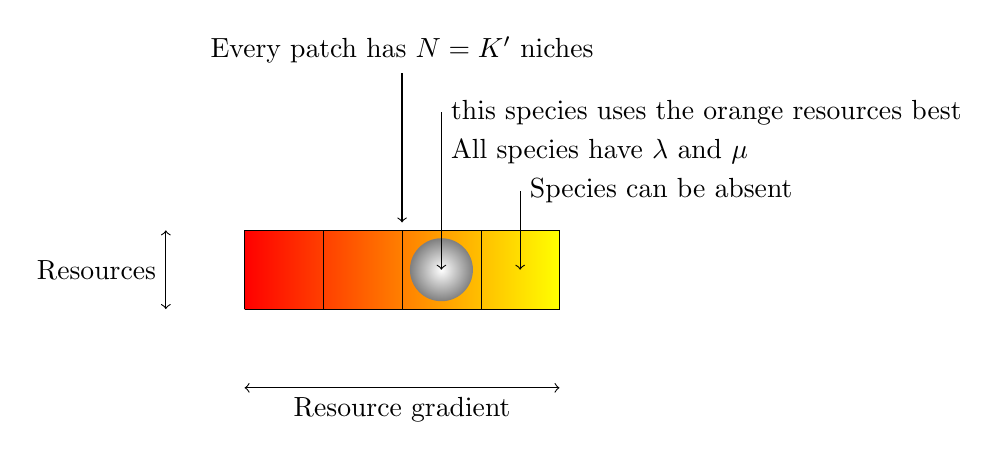
\begin{tikzpicture} 
  % Patch gradients
  \shade[left color=red,right color=yellow] (0,0) rectangle (4,1);
  % Species gradients
  \shade[inner color=white,outer color=gray] (2.5,0.5) circle (0.4 cm);
  % Grids
  \draw[step=1cm,black,very thin] (0,0) grid (4,1); 
  % Arrows
  \draw[<->] (0,-1) -- (2,-1) node[anchor=north] {Resource gradient} -- (4,-1) ;
  \draw[<->] (-1,0) -- (-1,0.5) node[anchor=east] {Resources} -- (-1,1) ;
  \draw[<-] (2,1+0.1) -- (2.0,3) node[anchor=south] {Every patch has $N = K'$ niches};
  \draw[<-] (2.5,0.5) 
    -- (2.5,2.5) node[anchor=west] {this species uses the orange resources best}
    -- (2.5,2) node[anchor=west] {All species have $\lambda$ and $\mu$};
  \draw[<-] (3.5,0.5) -- (3.5,1.5) node[anchor=west] {Species can be absent};
\end{tikzpicture}